%% LaTeX-Beamer template for KIT design
%% by Erik Burger, Christian Hammer
%% title picture by Klaus Krogmann
%%
%% version 2.1
%%
%% mostly compatible to KIT corporate design v2.0
%% http://intranet.kit.edu/gestaltungsrichtlinien.php
%%
%% Problems, bugs and comments to
%% burger@kit.edu

\documentclass[19pt]{beamer}

%% SLIDE FORMAT

% use 'beamerthemekit' for standard 4:3 ratio
% for widescreen slides (16:9), use 'beamerthemekitwide'

\usepackage{templates/beamerthemekit}
\usepackage{wrapfig}

\usepackage[utf8]{inputenc}
\usepackage[T1]{fontenc}
\usepackage[ngerman]{babel}	% german hyphenation, quotes, etc
\usepackage{tikz}
\usepackage{hyperref}
% \usepackage[ngerman]{translator}

% \usepackage{templates/beamerthemekitwide}

%% TITLE PICTURE

% if a custom picture is to be used on the title page, copy it into the 'logos'
% directory, in the line below, replace 'mypicture' with the 
% filename (without extension) and uncomment the following line
% (picture proportions: 63 : 20 for standard, 169 : 40 for wide
% *.eps format if you use latex+dvips+ps2pdf, 
% *.jpg/*.png/*.pdf if you use pdflatex)
\titleimage{Gruppenarbeit_klein}

%% TITLE LOGO

% for a custom logo on the front page, copy your file into the 'logos'
% directory, insert the filename in the line below and uncomment it

%\titlelogo{Logo_IOSB}

% (*.eps format if you use latex+dvips+ps2pdf,
% *.jpg/*.png/*.pdf if you use pdflatex)

%% TikZ INTEGRATION

% use these packages for PCM symbols and UML classes
% \usepackage{templates/tikzkit}
% \usepackage{templates/tikzuml}

% the presentation starts here

\title[PCC]{Privacy Crash Cam:\\ Entwurf}
\subtitle{App, Web-Interface und Web-Dienst}
\author{David L., Fabian W.}

\institute{Fraunhofer Institut f\"ur Optronik, Systemtechnik und Bildauswertung, (KIT)}

% Bibliography

\usepackage[citestyle=authoryear,bibstyle=numeric,hyperref,backend=biber]{biblatex}
\addbibresource{templates/example.bib}
\bibhang1em

\begin{document}

% change the following line to "ngerman" for German style date and logos
\selectlanguage{ngerman}

%title page
\begin{frame}
	\titlepage
\end{frame}

%###############################################################################################
%									Aufgabenstellung											  %
%###############################################################################################
\section{Aufgabenstellung}
\subsection{Szenario}
\begin{frame}{Szenario}
	\begin{center}
		%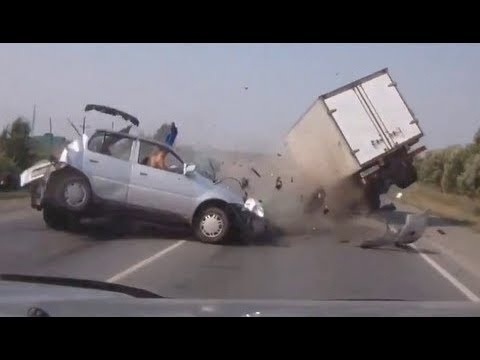
\includegraphics[scale=0.55]{logos/UnfallSzenario} 
		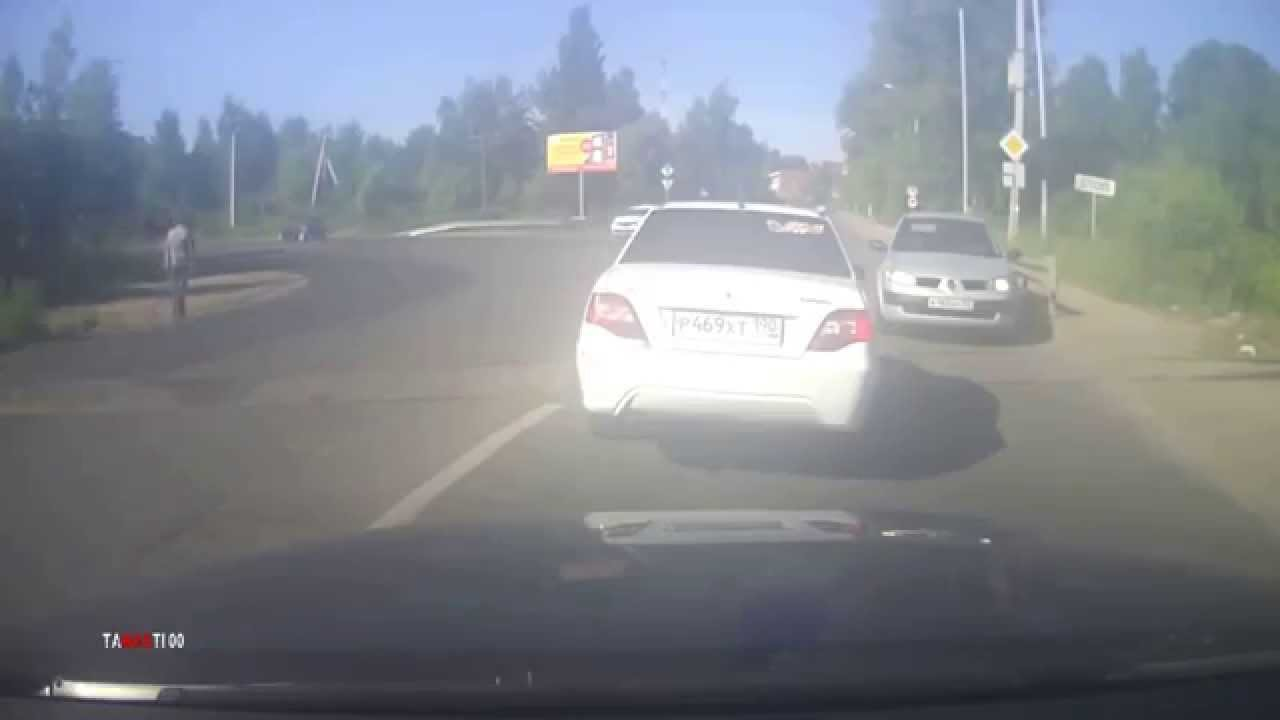
\includegraphics[scale=0.25]{logos/UnfallSzenario2} 
		%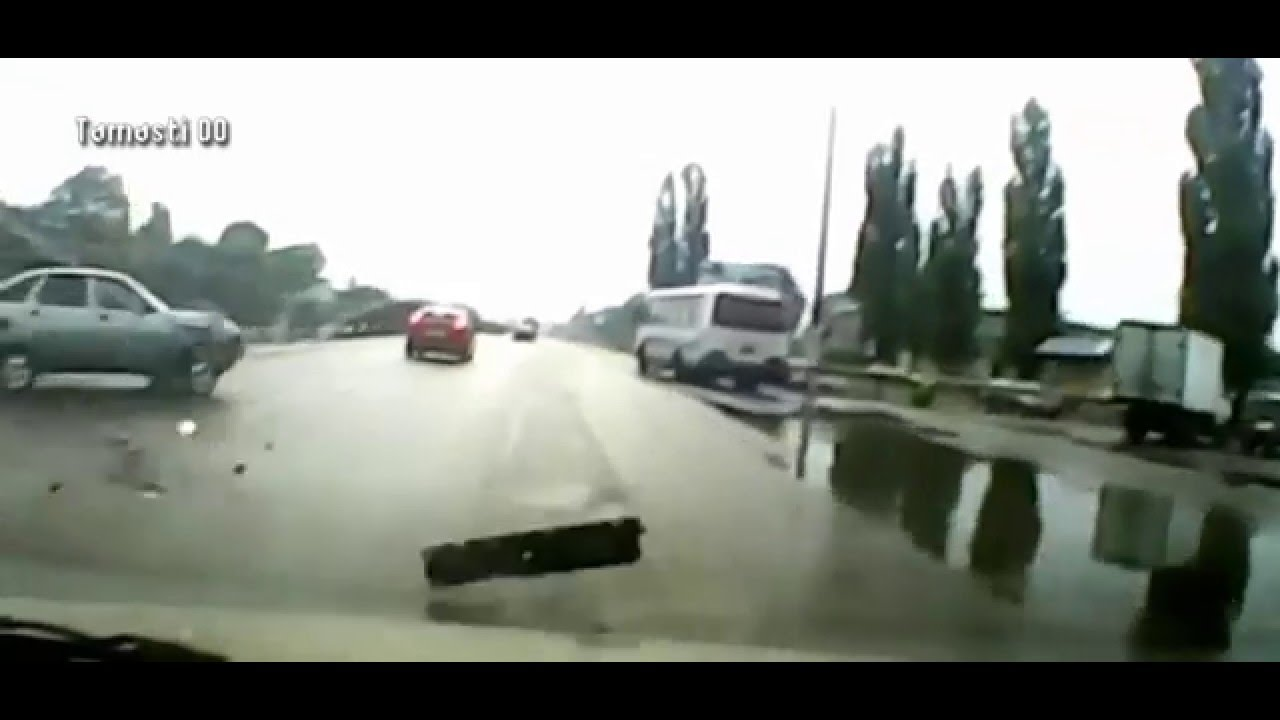
\includegraphics[scale=0.25]{logos/UnfallSzenario3} 
	\end{center}
\end{frame}

\subsection{Aufgabenstellung}
\begin{frame}{Aufgabenstellung}
	\begin{itemize}
		\item Verschl\"usselnde Crashcam-App
		\item Web-Interface zur Videoverwaltung
		\item Web-Dienst f\"ur Entschl\"usselung, Bildauswertung und Anonymisierung
	\end{itemize}
\end{frame}

\subsection{Aufgabenstellung - App}
\begin{frame}{Aufgabenstellung - App}
  \begin{columns}[T]
    \begin{column}{.5\textwidth}
    		\begin{itemize}
    			\item Ansichten
			\begin{itemize}
				\item Kamera
				\item Videos
				\item Einstellungen
			\end{itemize}
			\item 2 Kamera-Modi
			\begin{itemize}
				\item Beobachtungsmodus
				\begin{itemize}
					\item Ringpuffer (1 min)
				\end{itemize}
				\item Aufnahmemodus
				\begin{itemize}
					\item persistieren
					\item verschl\"usseln
				\end{itemize}
			\end{itemize}
			\item Verschl\"usselung
    		\end{itemize}
    \end{column}
    \begin{column}{.5\textwidth}
    		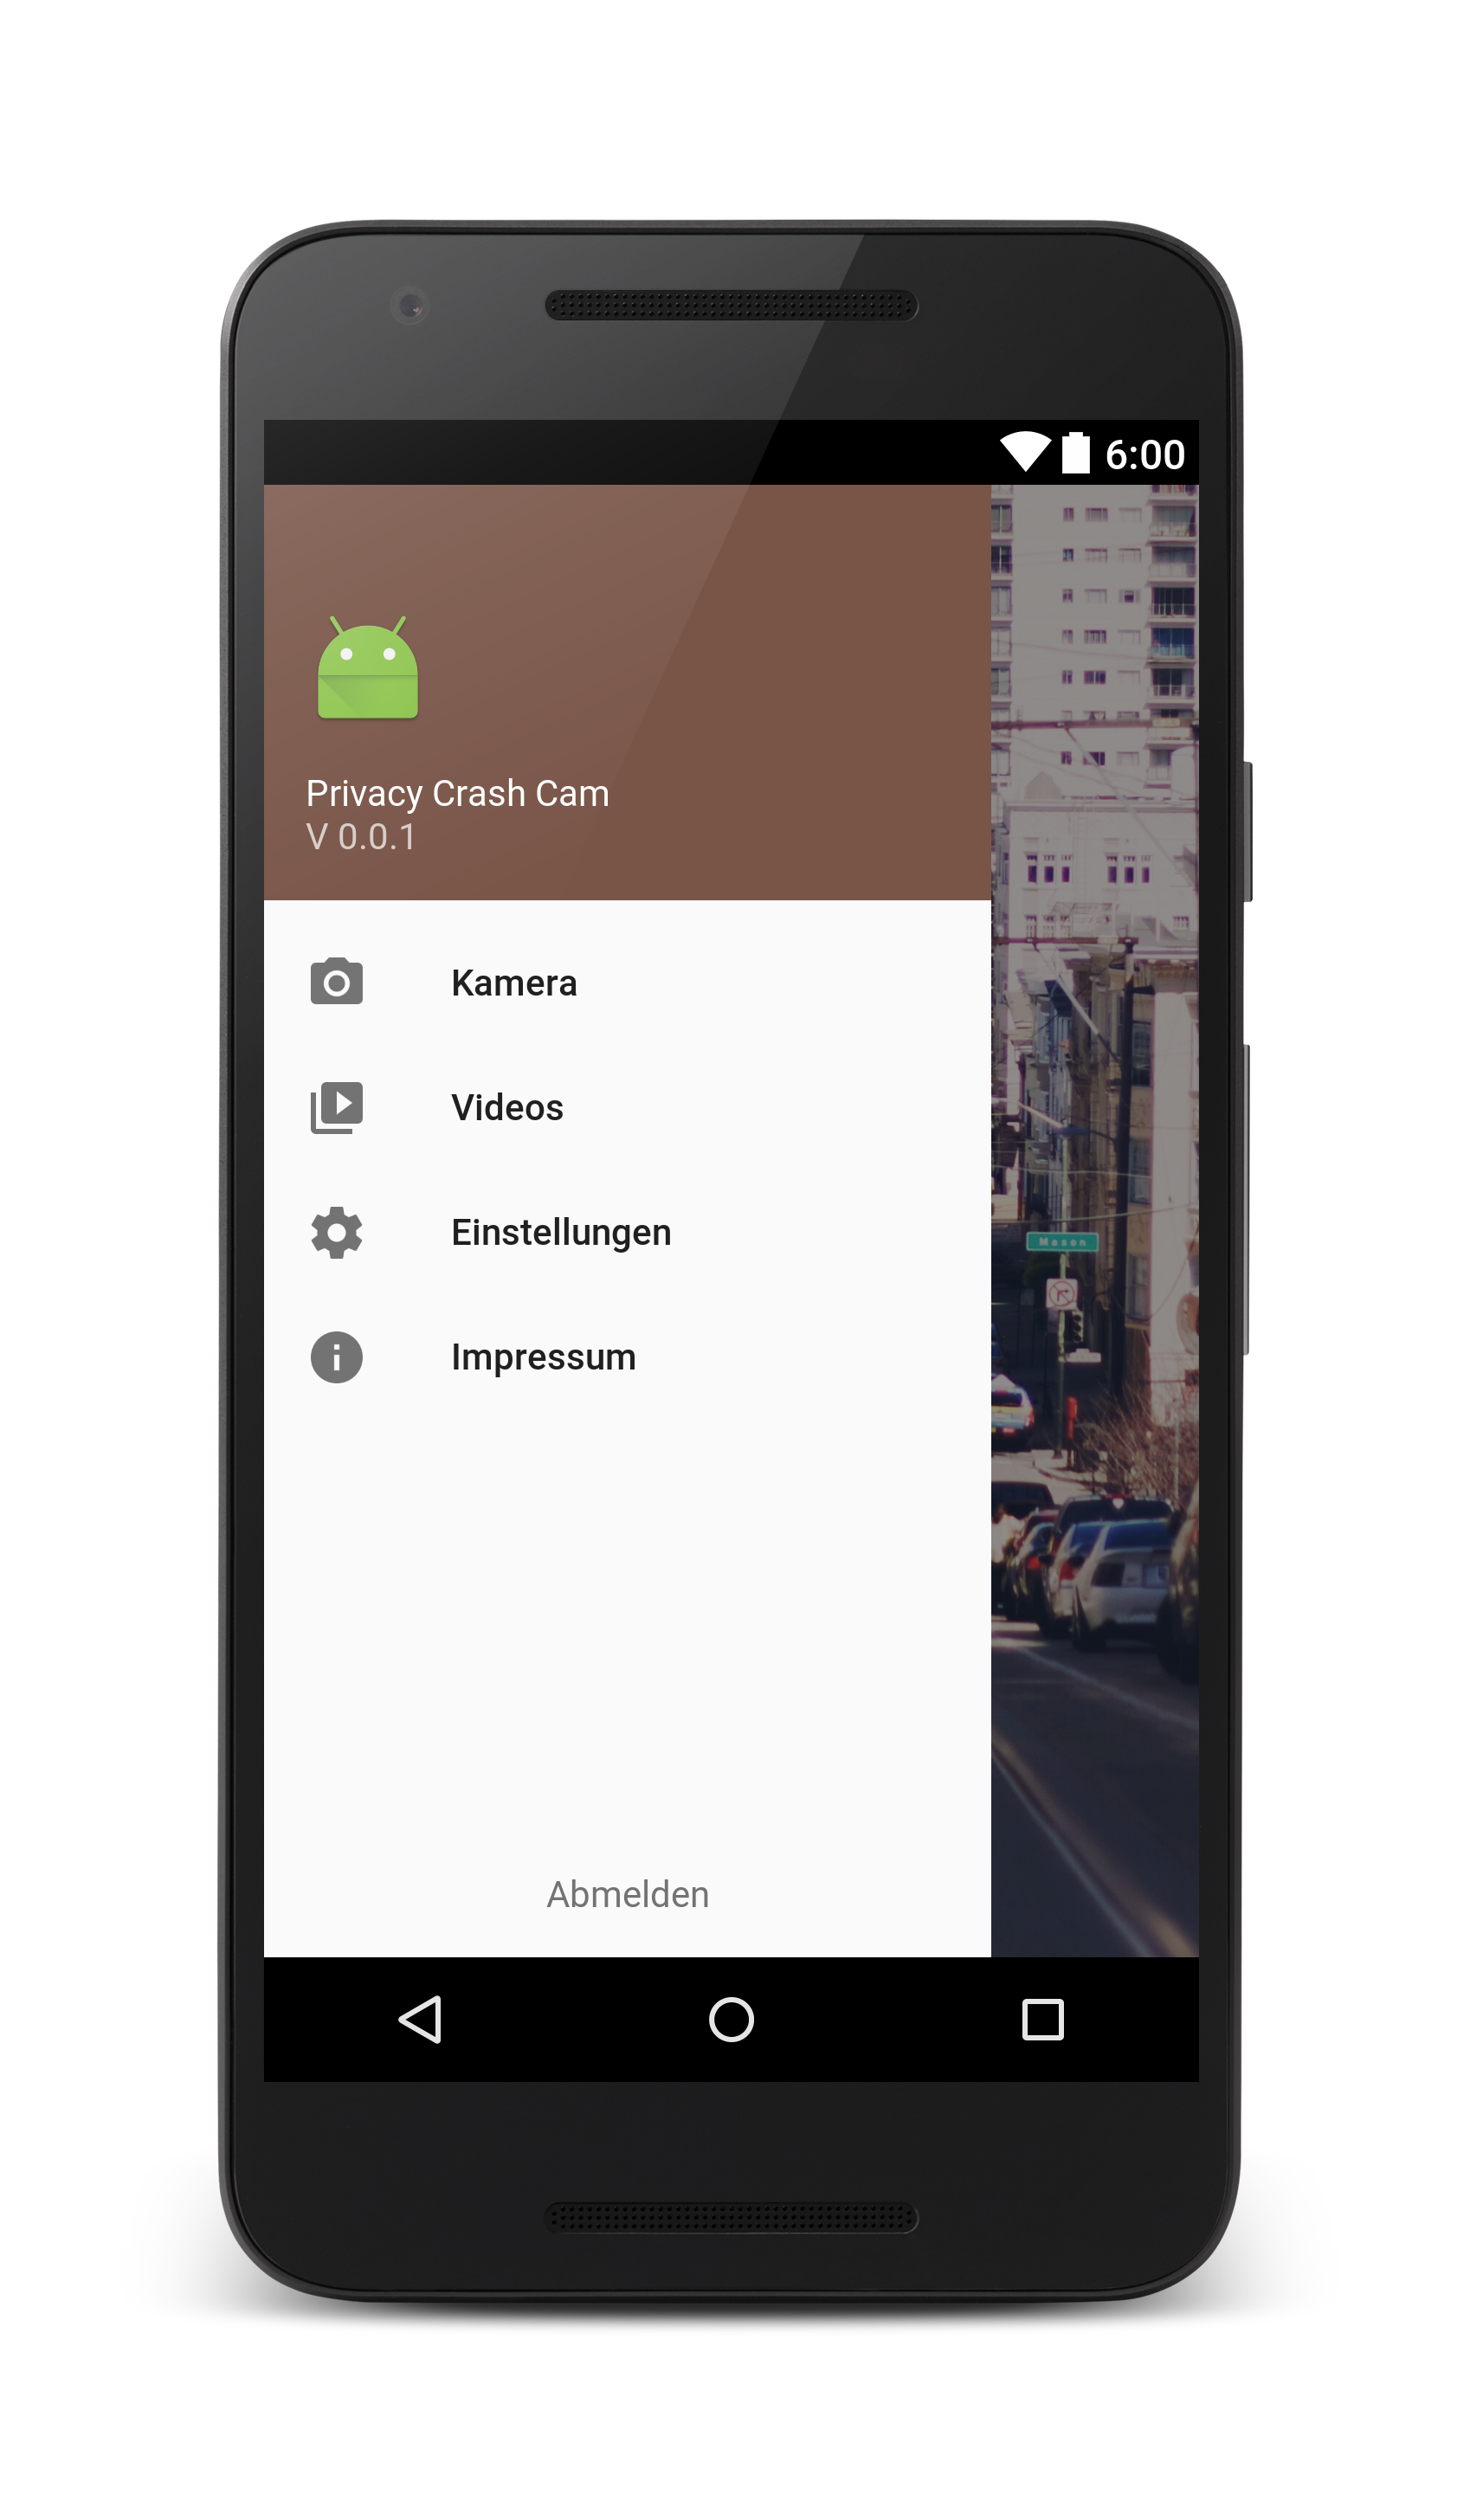
\includegraphics[scale=0.075]{logos/Mockups/Portrait_camera_view_menu_phone}
    \end{column}
  \end{columns}
\end{frame}


\subsection{Aufgabenstellung - Web-Interface}
\begin{frame}{Aufgabenstellung - Web-Interface}
  \begin{columns}[T]
    \begin{column}{.5\textwidth}
    		\begin{itemize}
    			\item Ansicht anonymisierter Videos
    			\begin{itemize}
					\item Herunterladen
					\item Info
					\item L\"oschen
				\end{itemize}
    			\item Accountverwaltung
    			\begin{itemize}
					\item Erstellen
					\item \"Andern
					\item L\"oschen
				\end{itemize}
    		\end{itemize}
    \end{column}
    \begin{column}{.5\textwidth}
    		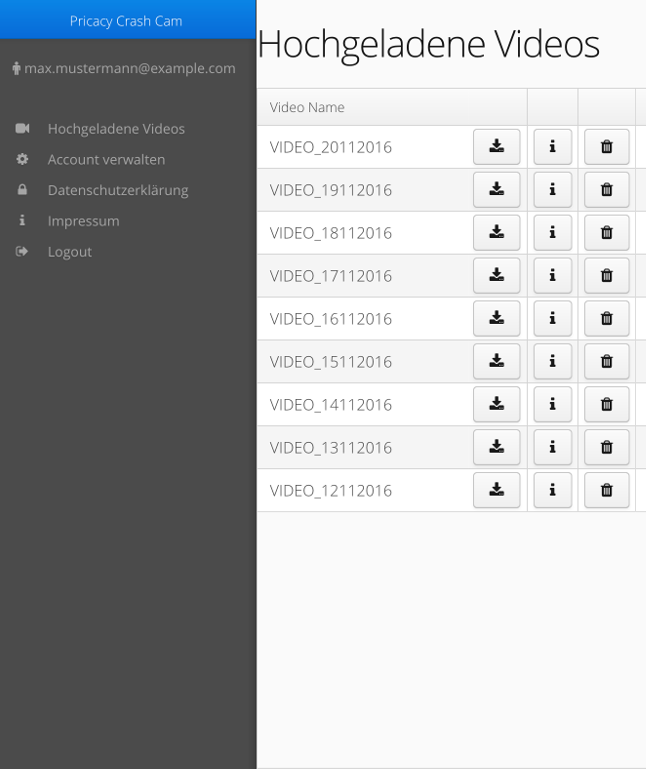
\includegraphics[scale=0.5]{logos/Mockups/Webinterface_small_pres}
    \end{column}
  \end{columns}
\end{frame}

\subsection{Aufgabenstellung - Web-Dienst}
\begin{frame}{Aufgabenstellung - Web-Dienst}
	\begin{itemize}
		\item Bearbeitet Anfragen der App und des Web-Interface
		\item Videoverarbeitung
			\begin{itemize}
				\item entschl\"usseln
				\item analysieren
				\item anonymisieren
			\end{itemize}
		\item Datenverwaltung
			\begin{itemize}
				\item Accountdaten
				\item Videodaten
			\end{itemize}
	\end{itemize}
\end{frame}

%###############################################################################################
%											Ziele											      %
%###############################################################################################

\section{Ziele}

\subsection{Ziele Entwurf - Allgemein}
\begin{frame}{Ziele Entwurf - Allgemein}
	\begin{itemize}
    	\item Modularisierung
		\begin{itemize}
			\item Reduzierte Koordination/Kommunikation
			\item Erhöhte Flexibilität
			\item Erhöhte Wiederverwertbarkeit
			\item Bessere Austauschbarkeit
		\end{itemize}
	\end{itemize}
\end{frame}

\subsection{Ziele Entwurf - Allgemein}
\begin{frame}{Model View Presenter (MVP)}
\begin{center}
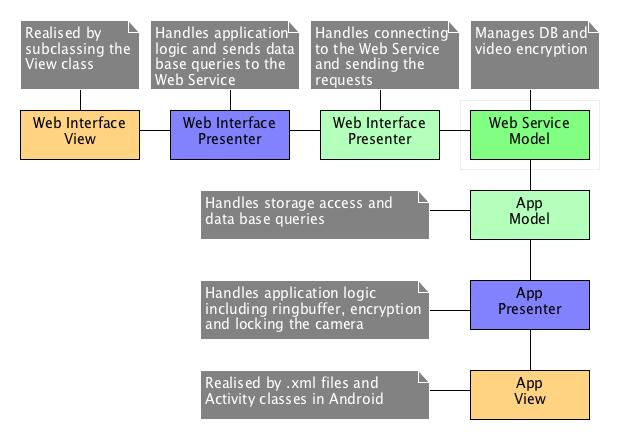
\includegraphics[scale=0.3]{resources/overview_mvp.jpg}
\end{center}
\end{frame}

\subsection{Ziele Entwurf - App}
\begin{frame}{Ziele Entwurf - App}
	\begin{itemize}
		\item GUI erweiterbar
		\item Datenverarbeitung, Netzwerkanfragen, Kamera austauschbar / abgeschottet
		\item Besondere Probleme
		\begin{itemize}
			\item Ringpuffer
			\item Asynchrone Vorgänge in Android
			\item Kamera-Handling + Austauschbarkeit
		\end{itemize}
	\end{itemize}
\end{frame}

\subsection{Ziele Entwurf - Web-Interface}
\begin{frame}{Ziele Entwurf - Web-Interface}
    \begin{itemize}
		\item Gute Usability
		\item Anzeige und Logik entkoppeln
    	\item Besondere Probleme
    	\begin{itemize}
			\item Entkoppeln von Logik und Anzeige
			\item Kommunikation mit dem Web-Dienst
			\item Vaadin
		\end{itemize}
    \end{itemize}
\end{frame}

\subsection{Ziele Entwurf - Web-Dienst}
\begin{frame}{Ziele Entwurf - Web-Dienst}
	\begin{itemize}
		\item Einheitliche Schnittstelle nach außen
		\item Authentifizierung bei jeder Anfrage
		\item Schnittstellen, Datenablage und Videoverarbeitung trennen
		\item Besondere Probleme
		\begin{itemize}
			\item Videoverarbeitung per Pipeline
			\item Großer Umfang an Funktionalität
			\item Schnittstelle
		\end{itemize}
	\end{itemize}
\end{frame}

%###############################################################################################
%											UML-Webdienst									      %
%###############################################################################################

\section{UML}
\subsection{Web-Dienst - UML \"{U}berblick}
\begin{frame}{Web-Dienst - UML \"{U}berblick}
\begin{center}
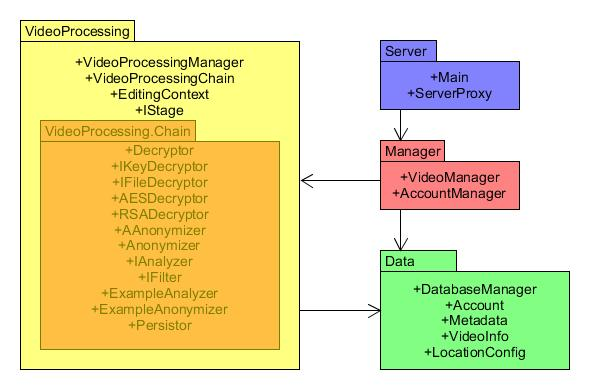
\includegraphics[scale=0.5]{resources/modules_overview_service.jpg}
\end{center}
\end{frame}
\subsection{Web-Dienst - UML Diagramm}
\begin{frame}{Web-Dienst - UML Diagramm}
\begin{center}
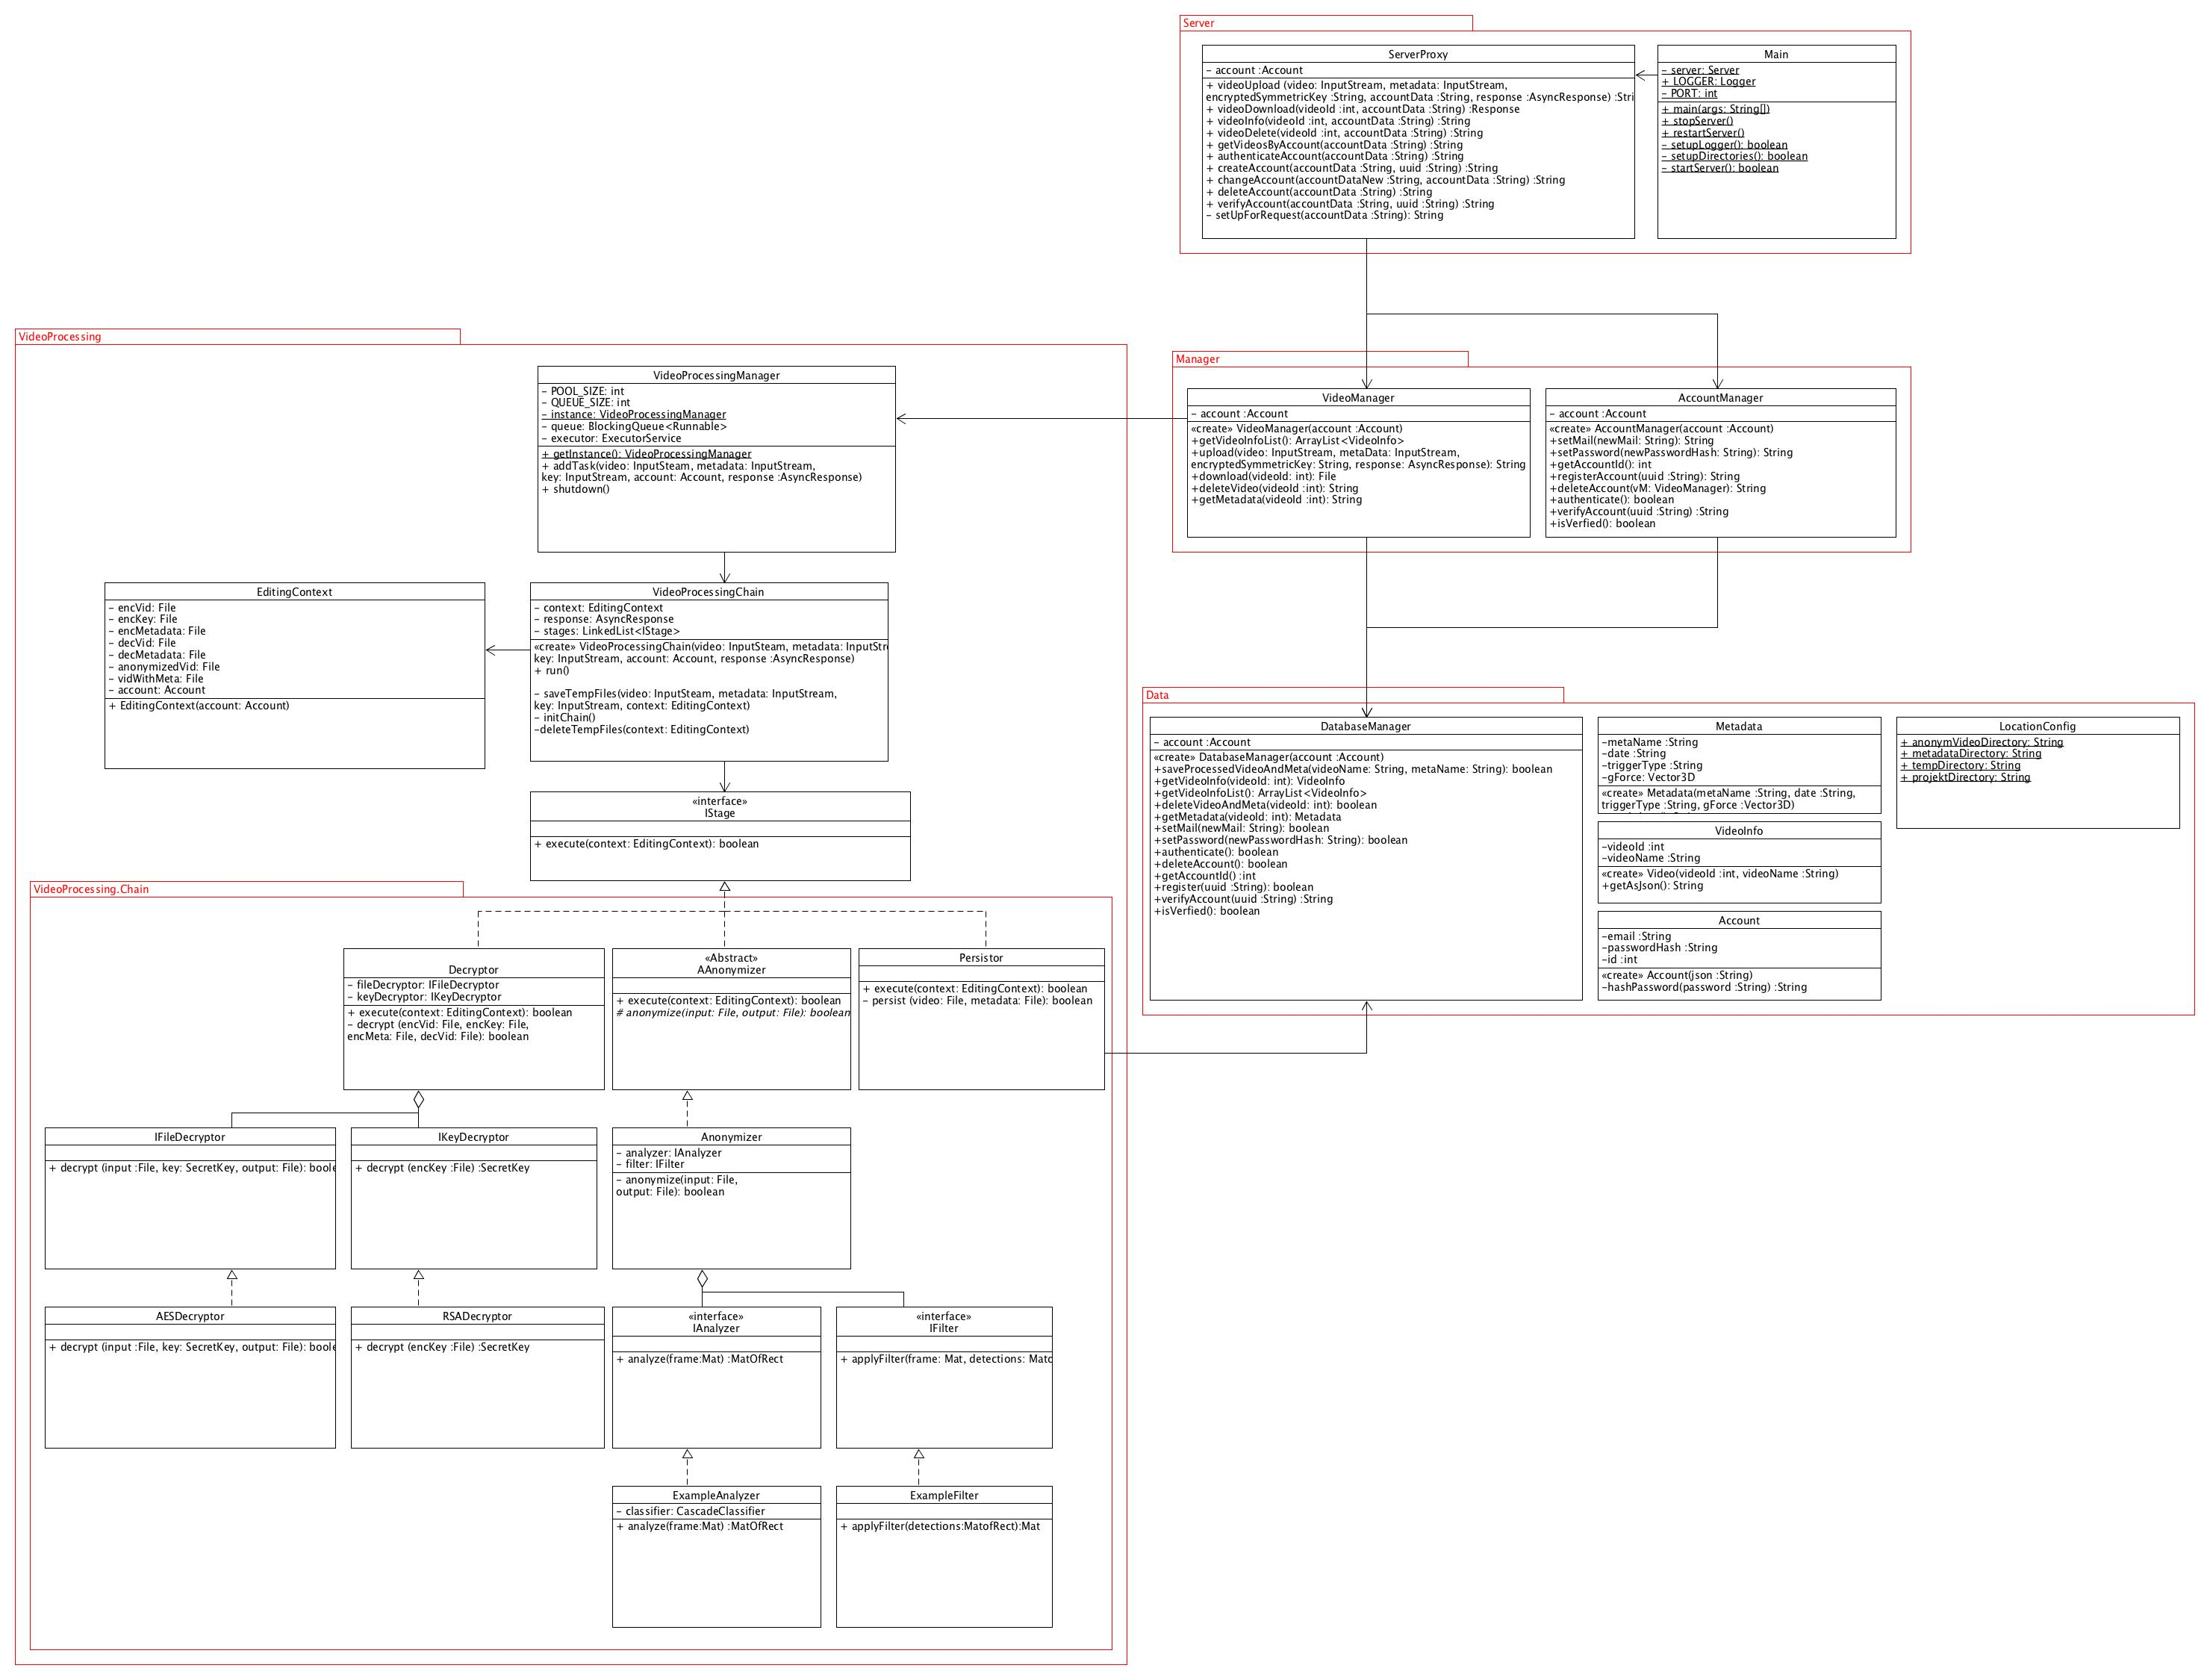
\includegraphics[scale=0.093]{resources/UMLSERVERPCC.jpg}
\end{center}
\end{frame}
\subsection{Web-Dienst - Schnittstelle}
\begin{frame}{Web-Dienst - Schnittstelle}
\begin{center}
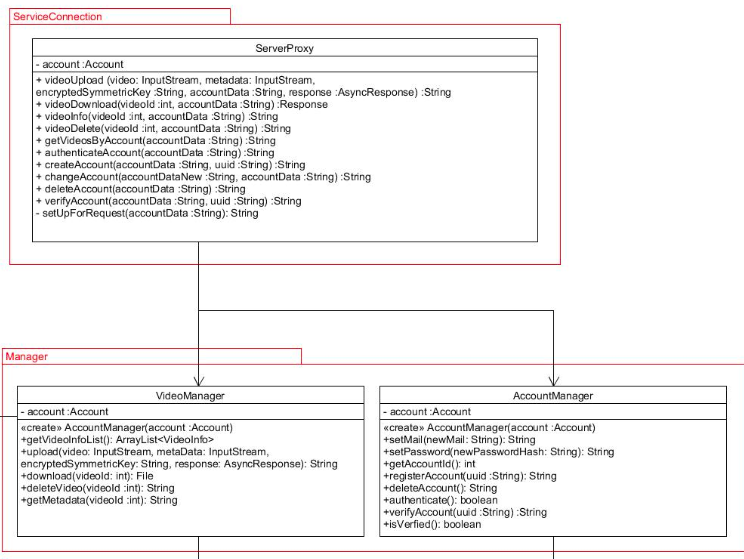
\includegraphics[scale=0.3]{resources/service_rest.png}
\end{center}
\end{frame}
\subsection{Web-Dienst - Datenbank}
\begin{frame}{Web-Dienst - Datenbank}
\begin{center}
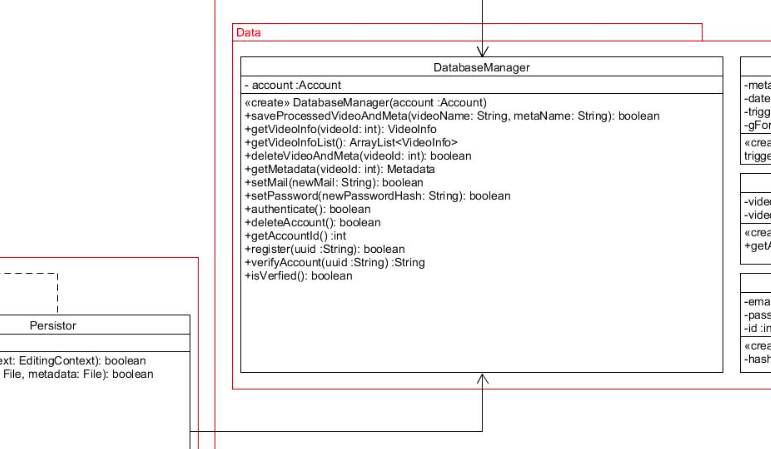
\includegraphics[scale=0.35]{resources/service_db.png}
\end{center}
\end{frame}
\subsection{Web-Dienst - Datenbank}
\begin{frame}{Web-Dienst - Datenbank}
\begin{center}
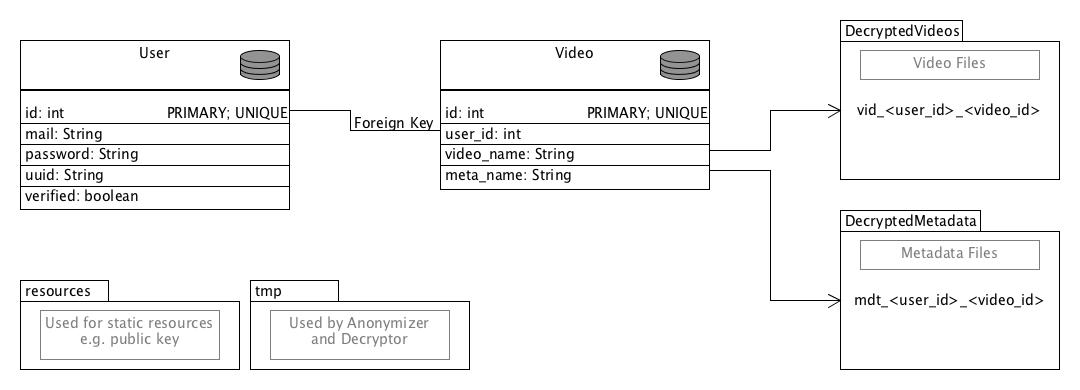
\includegraphics[scale=0.3]{resources/database_scheme.jpg}
\end{center}
\end{frame}
\subsection{Web-Dienst - Video Chain}
\begin{frame}{Web-Dienst - Video Chain}
\begin{center}
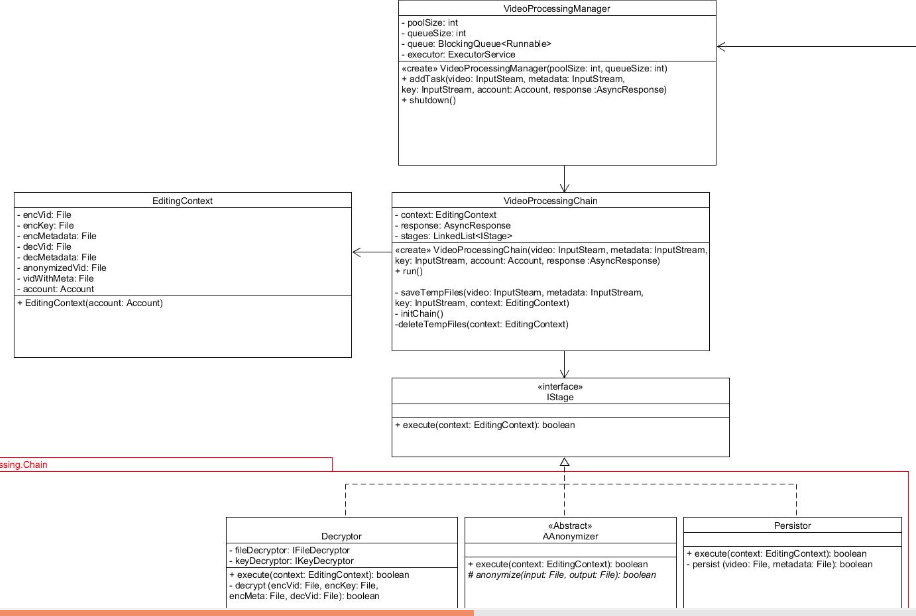
\includegraphics[scale=0.3]{resources/service_vidchain.png}
\end{center}
\end{frame}

%###############################################################################################
%											UML APP											      %
%###############################################################################################

\section{UML}
\subsection{App - UML \"{U}berblick}
\begin{frame}{App - UML \"{U}berblick}
\begin{center}
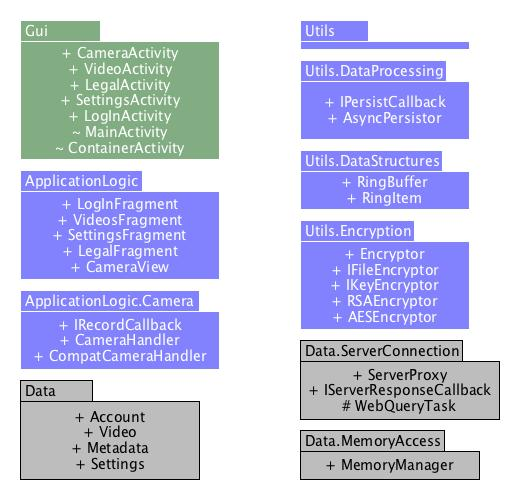
\includegraphics[scale=0.4]{resources/modules_overview_app.jpg}
\end{center}
\end{frame}
\subsection{App - UML Diagramm}
\begin{frame}{App - UML Diagramm}
\begin{center}
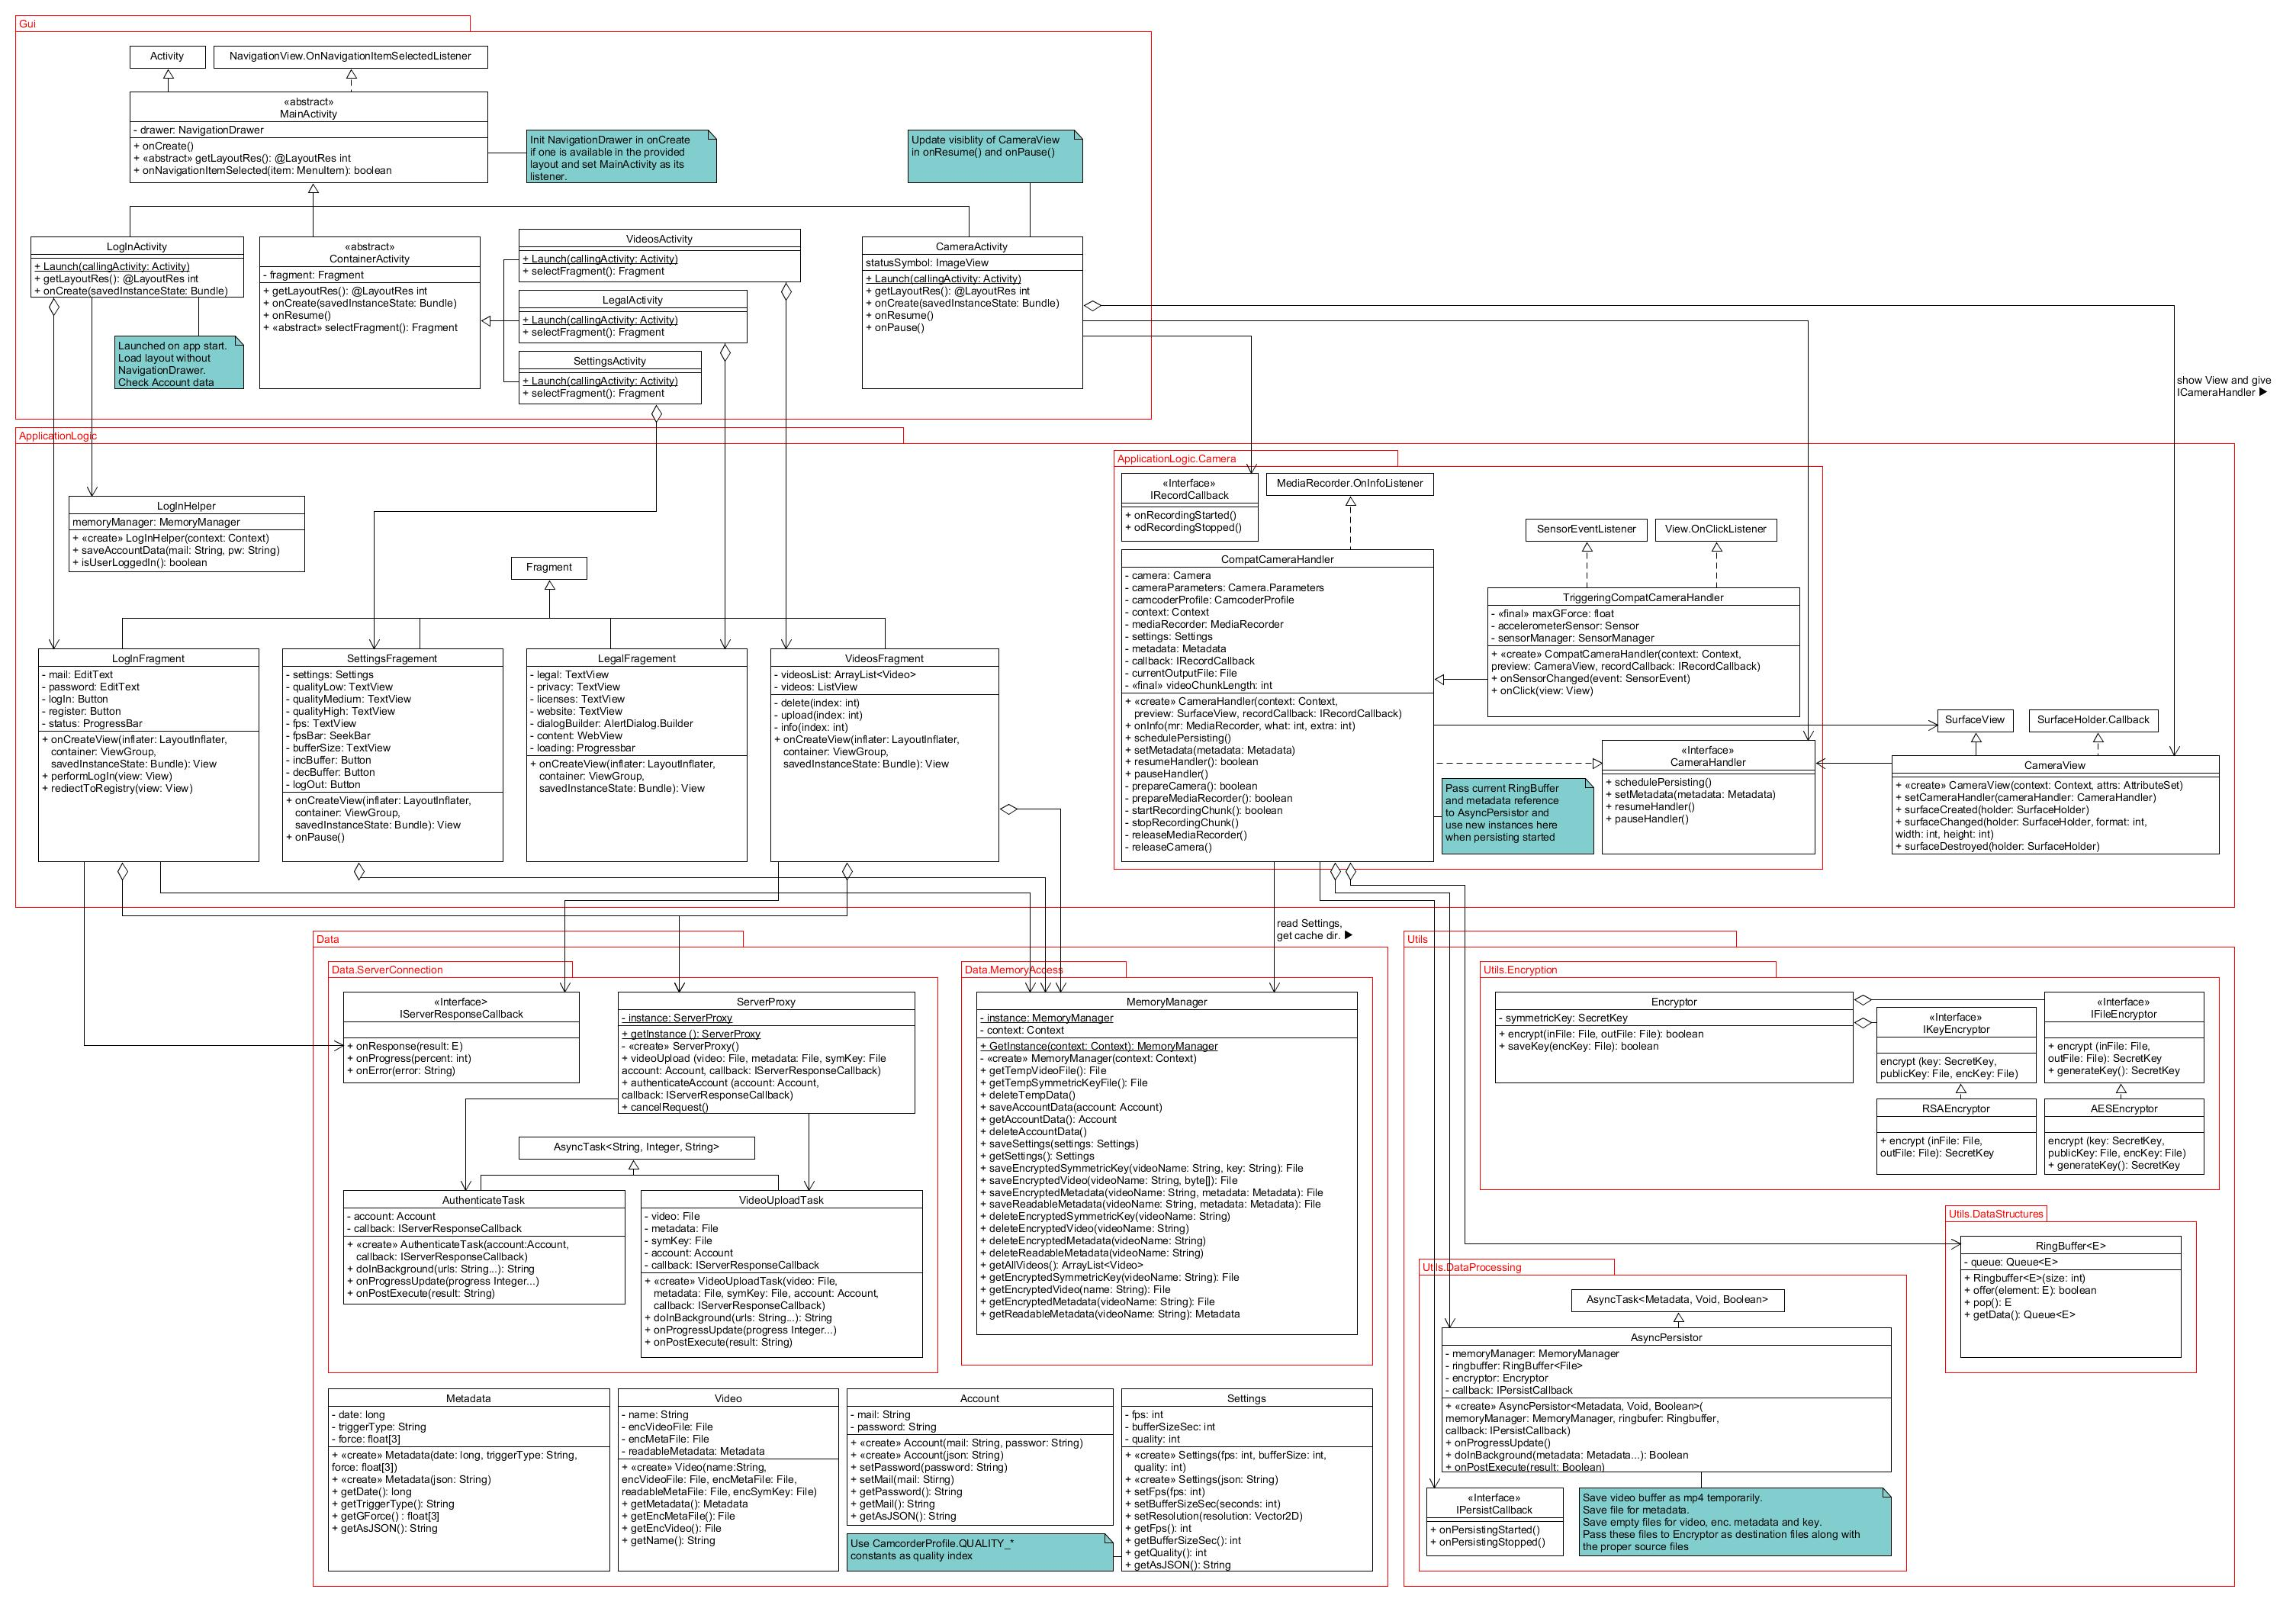
\includegraphics[scale=0.093]{resources/UMLAndroidApp.jpg}
\end{center}
\end{frame}
\subsection{App - GUI}
\begin{frame}{App - GUI}
\begin{center}
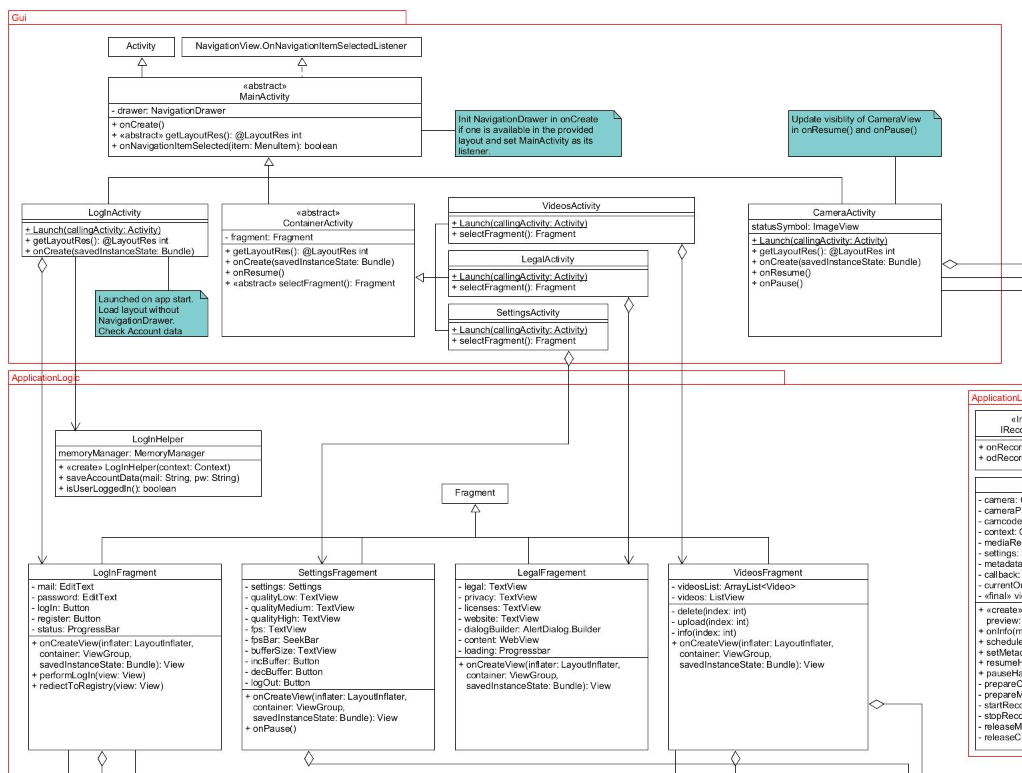
\includegraphics[scale=0.25]{resources/app_gui.png}
\end{center}
\end{frame}
\subsection{App - Application Logic}
\begin{frame}{App - Application Logic}
\begin{center}
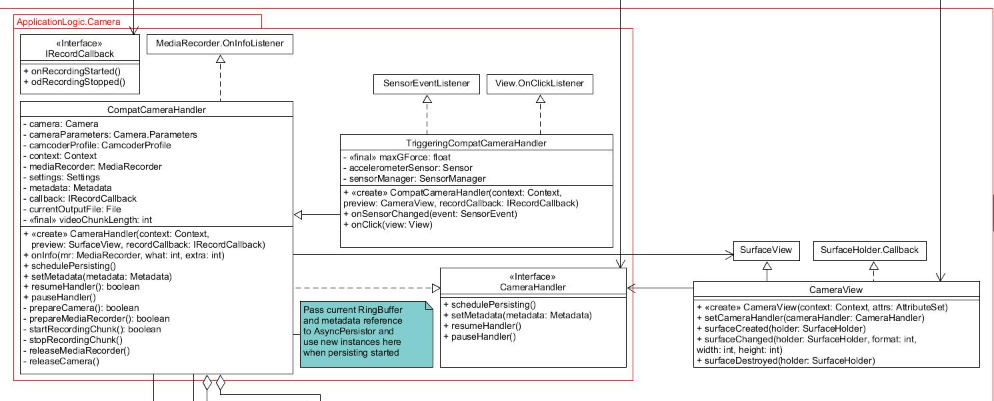
\includegraphics[scale=0.3]{resources/app_applogic.png}
\end{center}
\end{frame}
\subsection{App - Daten}
\begin{frame}{App - Daten}
\begin{center}
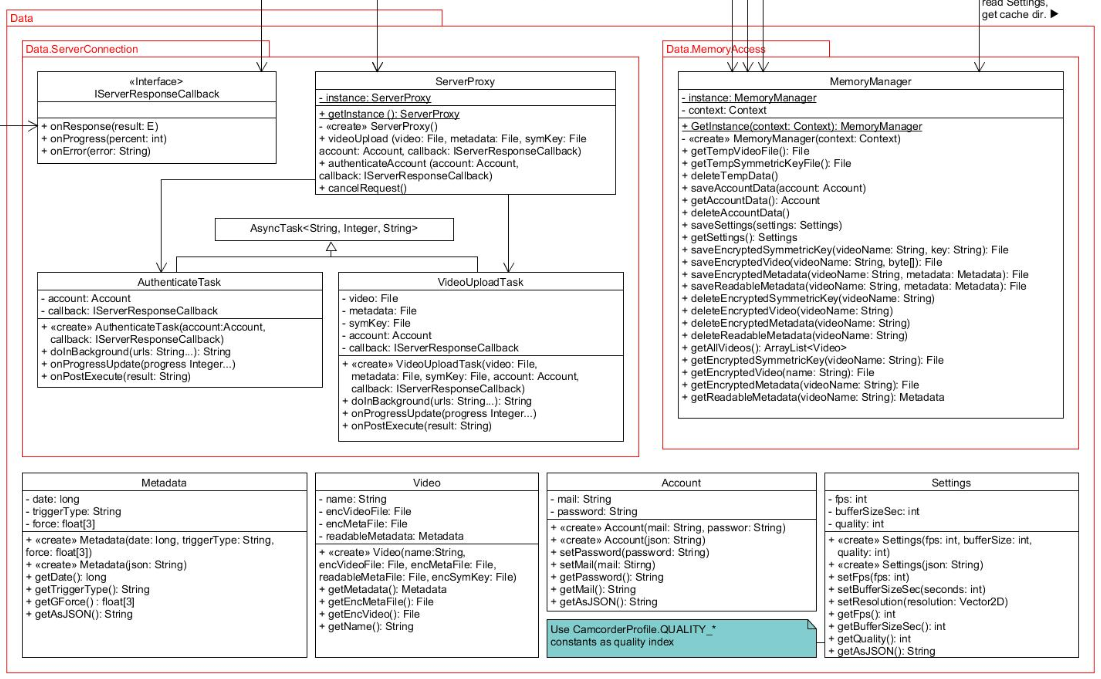
\includegraphics[scale=0.25]{resources/app_data.png}
\end{center}
\end{frame}
\subsection{App - Utils}
\begin{frame}{App - Utils}
\begin{center}
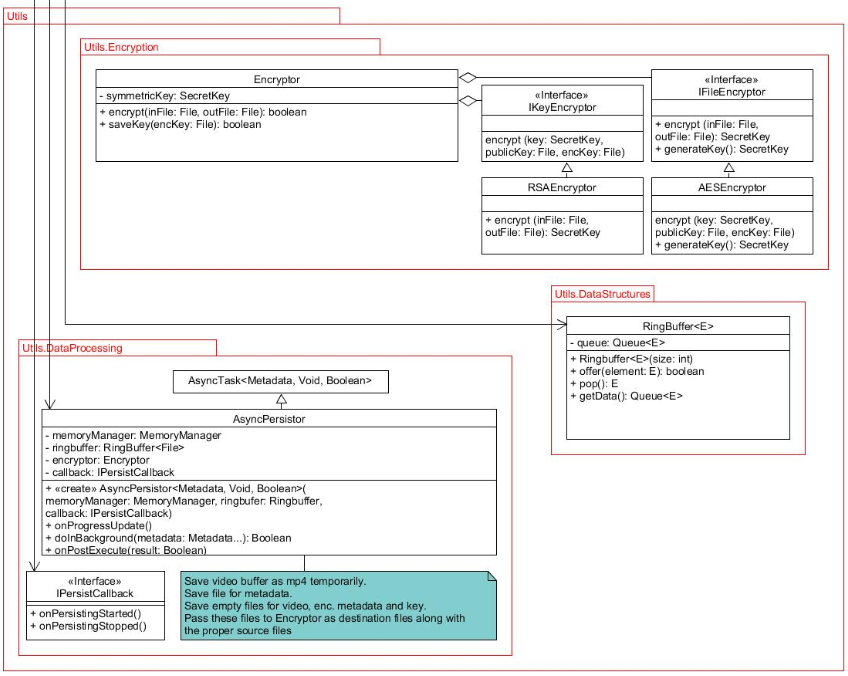
\includegraphics[scale=0.3]{resources/app_utils.png}
\end{center}
\end{frame}

%###############################################################################################
%											Github											      %
%###############################################################################################

\section{Github}
\subsection{Github - Einf\"{u}hrung}
\begin{frame}{Github - Einf\"{u}hrung}
\begin{itemize}
\item PSE Phasen in Git Repos \textbf{\href{https://github.com/rocklyve}{https://github.com/rocklyve}} \\

    	\begin{tabular}{| p{0.4\textwidth} | p{0.5\textwidth} |}
  			\hline			
  			Pflichtenheft & \textbf{\href{https://github.com/rocklyve/pcc-funcspec}{pcc-funcspec}}\\
  			\hline			
  			Entwurf & \textbf{\href{https://github.com/rocklyve/pcc-design}{pcc-design}}\\
  			\hline			
  			Implementierung 
  			\begin{itemize}
				\item App
				\item Web-Interface
				\item Web-Dienst
			\end{itemize} & \textbf{\href{https://github.com/rocklyve/pcc-imp}{pcc-imp}} \begin{itemize}
				\item \textbf{\href{https://github.com/rocklyve/pcc-imp-app}{pcc-imp-app}}
				\item \textbf{\href{https://github.com/rocklyve/pcc-imp-webinterface}{pcc-imp-webinterface}}
				\item \textbf{\href{https://github.com/rocklyve/pcc-imp-webservice}{pcc-imp-webservice}}
			\end{itemize}\\
  			\hline
  			Testphase & \textbf{\href{https://github.com/rocklyve/pcc-qa}{pcc-qa}}\\
  			\hline
  			Abschlusspr\"{a}sentation & \textbf{\href{https://github.com/rocklyve/pcc-present}{pcc-present}}\\
		  	\hline  
		\end{tabular}
	\end{itemize}
\end{frame}

%###############################################################################################
%											Demo											      %
%###############################################################################################

\section{Demo}
\begin{frame}{Demo}
	\begin{center}
		\textbf{DEMO}
	\end{center}
\end{frame}

%###############################################################################################
%											Ende											      %
%###############################################################################################

\begin{frame}{Ende}
	\begin{center}
		\textbf{Vielen Dank f\"{u}r eure Aufmerksamkeit} \\
		\textbf{Gibt es fragen?}
	\end{center}
\end{frame}

\end{document}
